% !TeX root = ../main-paper.tex
\section{Dataset}

%In this work, we  aim  at  producing  structured  spatio-temporal  data  from the information contained in the XIX\textsuperscript{th} century Parisian trade directories.
%To do this, it is therefore necessary to extract the text from the scans of the directories to be processed and to identify the entries in the various indexing lists used.
%Then, in each of these entries, the named entities they contain have to be extracted to produce structured spatio-temporal data representing the evolution over time of the people and businesses listed in these directories, their descriptions and their locations.
%Both of these extraction tasks require data to train and evaluate the OCR and NER approaches identified as potentially relevant: Tesseract and PERO OCR for the OCR task and Spacy and CamemBERT - pre-trained or fine-tuned - neural models for the NER task.

\subsection{The  XIX\textsuperscript{th} century Parisian trade directories}

The directories we have to process are stored in different libraries in Paris\footnote{Citer les bibliothèques sources?}. They have been scanned independently from each other and are available in digital format with various levels of quality. Moreover, they cover a wide period and ave been produced by different publishers and printers. Their contents, indexes, layouts, methods of printing, etc. vary thus from one directory to another (see Figure \ref{fig:directories}).


\begin{figure}[htb!]
	   \center{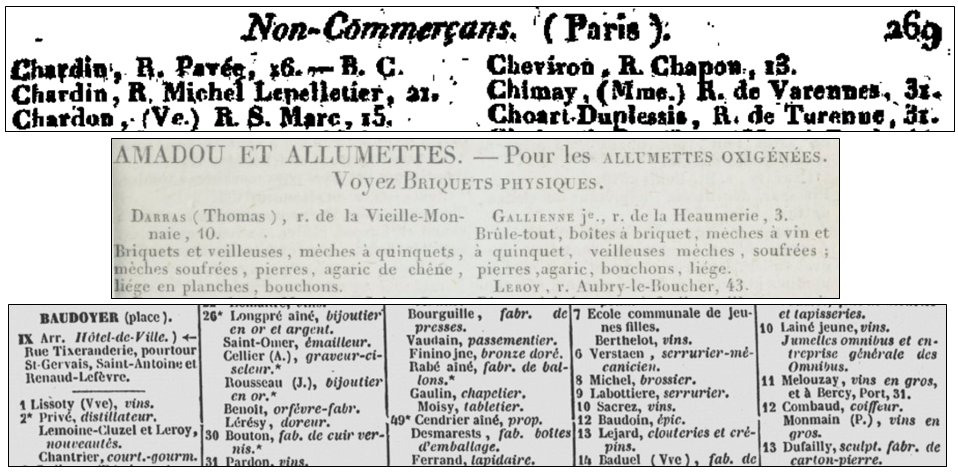
\includegraphics[width=0.9\textwidth]
	       {./images/DirectoryExcerpts2.png}}
	  \caption{\label{fig:directories} Examples of directory layouts and contents: 1) Duverneuil et La Tynna 1806 - index by name; 2) Deflandre 1828 - index by activity ; 3) Bottin 1851 –  index by street name}
\end{figure}


In this work, we therefore made a selection among the available directories, trying our best to retain copies representative of the diversity of existing directories and of sufficient quality to produce a reliable training data set. The Table \ref{tab:directories} lists the directories selected, their layout, the structure of their entries, and the number of annotated entries according to the indexes considered. For example, the Didot directory of 1854 is organised according to three indexes: by name, by activity, and by street name. The structure of the following entry is characteristic of its index by name: "Batton (D.-A.) *, professeur au Conservatoire de musique et de déclamation, Saint-Georges, 47." This entry begins with a person's name, followed by the initials of their first name in parentheses.The star symbol indicates that this person was awarded the Légion d'Honneur. The following part of this entry represents the person's activity,i.e. their profession, or social status, here "professor at the Conservatory of music and declamation". The street name and number where the person lives or carries out their activity are written at the end of the entry. These pieces of information constituting the structure of the entries are the basic data that we want to extract, deduplicate and structure in order to build a spatio-temporal database of XIX\textsuperscript{th} century Parisian inhabitants and businesses. With the exception of some potentially wordy activity descriptions, most of these pieces of information correspond to named entities. However, as Table \ref{tab:directories} shows, while most entries contain the same types of named entities, the order in which they appear and the way they are written vary from one directory to another. This argues for a supervised, rather than rule-based, NER approach, which requires annotated data.

\begin{table}[h!]
\resizebox{\textwidth}{!}{%
\begin{tabular}{|l|l|l|l|l|l|}
\hline
\multicolumn{1}{|c|}{\textbf{Directory publisher or name}} & \multicolumn{1}{c|}{\textbf{Year}} & \multicolumn{1}{c|}{\textbf{\# Col}} & \multicolumn{1}{c|}{\textbf{Index}} & \multicolumn{1}{c|}{\textbf{Entry structure}} & \multicolumn{1}{c|}{\textbf{\# Ann}}                                                                                                      
\\ \hline
Favre \& Duchesne & 1798 & 1 & by activity & {N [A], SN, SNUM - SEC.} & 233
\\ \hline
Duverneuil et La Tynna & 1801 & 1 & \begin{tabular}[c]{@{}l@{}}by activity\\ by name\end{tabular} & {N, SN, SNUM. SEC.} & \begin{tabular}[c]{@{}l@{}} 136 \\ 103\end{tabular}
\\ \hline
{Notables communaux de la Seine} & 1801 & 1 & by name & {N, [A,] SN[, SNUM].} & 92
\\ \hline
Duverneuil et La Tynna & 1805 &	2 &	\begin{tabular}[c]{@{}l@{}}by activity\\ by name\end{tabular} & \begin{tabular}[c]{@{}l@{}}N [(F)], SN, SNUM. - SEC.\\ N [(C)], [(A),] SN, SNUM. - SEC.\end{tabular} & \begin{tabular}[c]{@{}l@{}} 155 \\ 221 \end{tabular}
\\ \hline
Duverneuil et La Tynna & 1806 & 2 & \begin{tabular}[c]{@{}l@{}}by activity\\ by name\end{tabular} & \begin{tabular}[c]{@{}l@{}} N [(F)], SN, SNUM.\\ N [(C)], SN, SNUM.[ - SEC.]\end{tabular}. & \begin{tabular}[c]{@{}l@{}} 186\\ 0\end{tabular}
\\ \hline
La Tynna & 1813	& 2	& \begin{tabular}[c]{@{}l@{}}by activity\\ by name\end{tabular} & \begin{tabular}[c]{@{}l@{}} N,[A,] SN[, SNUM].\\ N, [(T)] A, SN[, SNUM] [, D].\end{tabular} & \begin{tabular}[c]{@{}l@{}} 135 \\ 177 \end{tabular}
\\ \hline
Panckoucke Commerces (Dulac) & 1820 & 1 & by name & N [(F)], A, [(T),] SN, SNUM[, P]. & 0
\\ \hline
Panckoucke Habitants (Dulac) & 1820	& 1 & by name & N [(T)], [A,] SN, SNUM [, D]. & 0
\\ \hline
Bottin (serie 1: 1819-1838) & 1820 & 2	& \begin{tabular}[c]{@{}l@{}}by activity\\ by name\end{tabular} & \begin{tabular}[c]{@{}l@{}} N [(F \textbar C)][T], [P], SN, SNUM.\\N [(F \textbar C)][T], A, SN, SNUM. CR\end{tabular} & \begin{tabular}[c]{@{}l@{}} 128 \\ 151 \end{tabular}
\\ \hline
Bottin (serie 1: 1819-1838) & 1827 & 2	& \begin{tabular}[c]{@{}l@{}}by activity\\ by name\end{tabular} & \begin{tabular}[c]{@{}l@{}}N [(F \textbar C)][T], [P], SN, SNUM.\\ N [(F \textbar C)][T], A, SN, SNUM.\end{tabular} & \begin{tabular}[c]{@{}l@{}} 228 \\ 285 \end{tabular}
\\ \hline
Deflandre & 1828 & 2 & \begin{tabular}[c]{@{}l@{}}by activity\\ by name\end{tabular} & \begin{tabular}[c]{@{}l@{}} N [(F \textbar C)][T], [P], SN, SNUM. \\N [(F \textbar C)][T], A, SN, SNUM.\end{tabular} & \begin{tabular}[c]{@{}l@{}}115\\ 229\end{tabular}
\\ \hline
Deflandre & 1829 & 2 & \begin{tabular}[c]{@{}l@{}}by activity\\ by name\end{tabular} & \begin{tabular}[c]{@{}l@{}}N [(F \textbar C)][T], [P], SN, SNUM.\\ N [(F \textbar C)][T], A, SN, SNUM.\end{tabular} & \begin{tabular}[c]{@{}l@{}}177\\ 236\end{tabular}
\\ \hline 
Bottin (serie 1: 1819-1838) & 1837 & 2	& \begin{tabular}[c]{@{}l@{}}by activity\\ by name\end{tabular} & \begin{tabular}[c]{@{}l@{}}N [(F \textbar C)][T], [P], SN, SNUM.\\ N [(F \textbar C)][T], [A], SN, SNUM.\end{tabular} & \begin{tabular}[c]{@{}l@{}}158\\ 557\end{tabular}
\\ \hline
Cambon - Almanach général & 1841 & 2 &	\begin{tabular}[c]{@{}l@{}}by activity\\ by name\end{tabular} & \begin{tabular}[c]{@{}l@{}}N [(F \textbar C)][T], [P], SN, SNUM.\\ N [(F \textbar C)][T], A, SN, SNUM.\end{tabular} & \begin{tabular}[c]{@{}l@{}}182\\ 486\end{tabular}
\\ \hline
Didot & 1841a &	\begin{tabular}[c]{@{}l@{}}3\\ 4\end{tabular} &	\begin{tabular}[c]{@{}l@{}}by activity \\ by name \end{tabular} & 	\begin{tabular}[c]{@{}l@{}}N [(F \textbar C)][T], [P], SN, SNUM. \\ N [(F \textbar C)][T], [A], SN, SNUM. \end{tabular} & \begin{tabular}[c]{@{}l@{}}246\\ 843\end{tabular}
\\ \hline
Didot & 1851a & \begin{tabular}[c]{@{}l@{}l@{}}4\\ 4\\ 5\end{tabular} & \begin{tabular}[c]{@{}l@{}l@{}}by activity\\ by name\\ by street name\end{tabular} & \begin{tabular}[c]{@{}l@{}l@{}}N [(F \textbar C)][T], [P], SN, SNUM.\\ N [(F \textbar C)][T], [A], SN, SNUM.\\SNUM N [(F \textbar C)][T], [A].\end{tabular} & \begin{tabular}[c]{@{}l@{}l@{}}309\\ 961\\ 0\end{tabular}
\\ \hline
Didot & 1854a & \begin{tabular}[c]{@{}l@{}l@{}}4\\ 3\\ 5\end{tabular} &	\begin{tabular}[c]{@{}l@{}l@{}} by activity \\ by name \\ by street name\end{tabular} & \begin{tabular}[c]{@{}l@{}l@{}} N [(F \textbar C)], [P], SN, SNUM [,T].\\ N [(F \textbar C)][T], [A], SN, SNUM.\\ SNUM N [(F \textbar C)][T], [A].\end{tabular} & \begin{tabular}[c]{@{}l@{}l@{}}106\\ 362\\ 0\end{tabular}
\\ \hline
Bottin (serie 3: 1854-1856) & 1854a & \begin{tabular}[c]{@{}l@{}l@{}}3\\ 2\\ 4\end{tabular} & \begin{tabular}[c]{@{}l@{}l@{}} by activity \\ by name \\ by street name\end{tabular} & \begin{tabular}[c]{@{}l@{}l@{}}N [(F \textbar C)], [P], SN, SNUM [,T].\\ N [(F \textbar C)][T], [A], SN, SNUM.\\ SNUM N [(F \textbar C)], [A] [,T].\end{tabular} & \begin{tabular}[c]{@{}l@{}l@{}}253\\ 633\\ 0\end{tabular}
\\ \hline
Didot-Bottin & 1860a	& 3	& by name & N [(F \textbar C)][T], [A], SN, SNUM. & 378
\\ \hline
Didot-Bottin & 1861a	& 3	& by name & N [(F \textbar C)][T], [A], SN, SNUM. & 402
\\ \hline
\end{tabular}%
}
\caption{The directories used to build our dataset. Letters next to year of publication are used to identify the volume of the directory. \# Col stands for "Number of columns", and \# Ann stands for "Number of annotated entries". Entry structure is described as follows: N - entry name (person or business); F - first name; T - honorary title; C - civility; A - activity; P - precision; SN - street name; SNUM - street number; SEC - section; D - district; CR - cross-reference; bracketed elements are optional.}
\label{tab:directories}
\end{table}

\subsection{Groundtruth data extraction}

Présenter ici l'outil d'annotation et le guide d'annotation suivi.


\subsection{Assessing the groundtruth quality}

Our dataset is thus made of excerpts 

TODO interesting points to detail:
\begin{itemize}
    \item origin
    \item illustration (maybe in first figure)
    \item various numbers (of the original data and of the sample we extracted) : number of entries per pages, variety of directory entries, \dots
    \item statistics about entry lengths (histogram of number of char / tokens par entry)
    \item entities we considered and how we annotated them (how we assessed gold's quality)
    \item statistics on the distribution of entities across directories and their arrangement within entries
    \item OCR data (automated systems and clean text + how we created the "clean" text + whether/how we assessed clean text's quality)
    \item Measure inter-annotator agreement ? 
    \item Explain charset projection
    \item \dots
\end{itemize}
